\documentclass[a4paper,11pt]{report}
\usepackage[T1]{fontenc}
\usepackage[utf8]{inputenc}
\usepackage{lmodern}
\usepackage[spanish]{babel}
\usepackage{graphicx} % para insertar graficos/imagenes
\usepackage{float} % me deja usar la H de 'here' en los graficos para ponerlos donde yo quiera
\usepackage{fancyhdr} % headers y footers
\usepackage{color} %Para colores y eso
\usepackage{geometry} %Para cambiar la geometria de las hojas
 \usepackage[hidelinks]{hyperref} 
\let\olditemize\itemize
\def\itemize{\olditemize\itemsep=0pt }

\title{Trabajo Practico: Fine Food Reviews\\Organización de Datos 75.06}
\author{Joaquín Blanco, Padrón: 94653\\
Joaquín Casal, Padrón: 98280\\
Franco Etcheverri, Padrón: 95812\\
Agustín Luques, Padrón: 96803\\
Nombre del grupo en Kaggle: Tony Spark}

\begin{document}

\maketitle
\tableofcontents

\begin{abstract}
En el presente trabajo se propone una estrategia para el análisis de reviews y la predicción de su puntaje en función de sus datos. Durante nuestra investigación realizamos un relevamiento del set de datos y se concluyo que uno de los campos mas importantes y sobre el cual basaremos gran parte de nuestro proyecto es el texto. 

Para poder explotar al máximo este recurso nos adentramos en una reciente área de estudio de las ciencias de la computación, el Text Mining. La misma combina técnicas del data mining, machine learning, procesamiento del lenguaje natural e informacion retrieval, áreas que están incluidas dentro de nuestro estudio y forman parte de la solución final. 

En términos generales, nuestra aplicación es la combinación de resultados de distintos clasificadores, los cuales serán expuestos a lo largo del informe, esperando que de esta forma, la precisión de nuestra predicción supere al de los clasificadores ejecutados de forma individual. 
\end{abstract}

\chapter{Análisis inicial de los datos}
En este capitulo nos dedicaremos a explorar el set de datos que tenemos a nuestra disposición. Los campos que incluyen cada uno de los registros del Train son los siguientes:

\begin{itemize}
  \item id: El id que identifica a cada review.
  \item ProductId: El Id del producto.
  \item UserId: El Id del usuario.
  \item ProfileName: El nombre del usuario. 
  \item HelpfulnessNumerator: El numerador indicando la cantidad de usuarios que juzgaron al review como util.
  \item HelpfulnessDenominator: El denominador indicando la cantidad de usuarios que evaluaron si el review fue útil o no.
  \item Prediction: La cantidad de estrellas del review.
  \item Time: Un timestamp para el review.
  \item Summary: Un resumen del review.
  \item Text: Texto del review.
\end{itemize}
En principio se descartaron del procesamiento de los datos los campos de ProductId, UserId, ProfileName y Time, ya que en un primer análisis no los consideramos con igual relevancia que el resto de los campos del review. Esto no descarta que en el caso de encontrar algún patrón claro que ayude a determinar los puntajes finales no se tomen en cuenta a posterior.

Denominaremos “Helpfulness Numbers” al conjunto que incluye tanto al HelpfulnessNumerator como al HelpfulnessDenominator. Este es un parámetro de gran importancia para ponderar el peso de cada review, ya que dan conocimiento de la credibilidad del comentario en cuestión. Aquellas reviews que tengan mayor proporción de votos positivos, representados como HelpfulnessNumerator, deberían tener mayor influencia en el resultado final de la predicción. Una forma de lograr esto es obteniendo el cociente entre ambos Helpfulness Numbers y utilizar dicho número como “función peso” y a partir de ella modificar el puntaje asignado. Mas tarde, este parámetro tomara relevancia como parte de un algoritmo de clasificación.

Teniendo en cuenta esto, quisimos analizar si había alguna tendencia en las reviews cuyo cociente entre los Helpfulness Numbers era muy bajo, ya que son a las que se les dará menor importancia.
A continuación, un gráfico que muestra la cantidad de reviews por puntaje, teniendo en cuenta solo reviews cuyo cociente era menor a 0.3 (se descartaron los casos en los que la review no tenía ningún voto)

\begin{figure}[htp]
  \begin{center}
    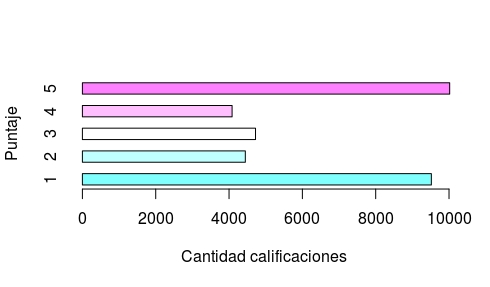
\includegraphics[width=10cm]{puntajcantfilter}
    \caption{Frecuencia de puntaje en review cuya Helpfulness Numbers es menor a 0.3}
    \label{fig:3}
  \end{center}
\end{figure}

Como se puede apreciar en la Figura \ref{fig:3}, las reviews con bajo cociente de Helpfulness Numbers tienen cierta tendencia a ser reviews con muy buenas o muy malas calificaciones (sugiriendo que los votantes no encuentran útiles las reviews cuyo autor consideró que todo era muy bueno o muy malo). Pero no existe una tendencia muy marcada hacia uno de los valores posibles para las calificaciones, por lo que darle menor peso a estas reviews no debería desbalancear los puntajes a otorgar cuando se hagan predicciones.

\begin{figure}[htp]
  \begin{center}
    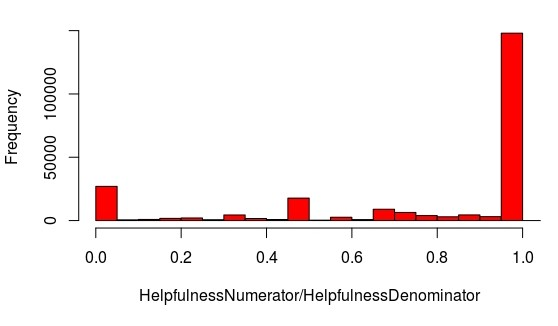
\includegraphics[width=10cm]{helpfullnesnumden}
    \caption{Histograma que muestra la frecuencia de los valores HelpfulnessNumerator/HelpfulnessDenominator}
    \label{fig:1}
  \end{center}
\end{figure}

En la Figura \ref{fig:1} podemos observar la dispersión de los datos con una mayor tendencia hacía reviews más creíbles. Pero un detalle no menor es que en este primer análisis no se consideraron casos puntuales que pueden llevar a una conclusión errónea.
Los únicos casos filtrados hasta aquí habían sido aquellos en los cuales no existian votos ni positivos ni negativos. Nuestro enfoque nos llevo a querer descartar aquellos reviews con pocos votos ya que no aseguran que el resultado de la división sea efectivamente acertado. Para ellos se ajusto el cálculo efectuado de la siguiente forma:
\[ 
   \left \{
      \begin{array}{lcccl}
         0 & si & HelpfulnessDenominator < X\\ 
         Helpfulness Numerator/Helpfulness Denominator  & si & X < HelpfulnessDenominator < Y\\ 
         Helpfulness Numerator/Helpfulness Denominator  \cdot \delta & si & Y < HelpfulnessDenominator
      \end{array}
   \right .
 \]
Donde $\delta > 1$ es un factor que le otorga mayor peso a los reviews con una cantidad de votos elevados. X e Y van a ser determinados luego de analizar en detalle la cantidad de votos por review en el total del set de datos.

Para tener una primer idea de los posibles resultados, analizamos la cantidad de registros por cada valor posible de estrellas y lo que obtuvimos se puede observar en la Figura \ref{fig:2}. 

\begin{figure}[htp]
  \begin{center}
    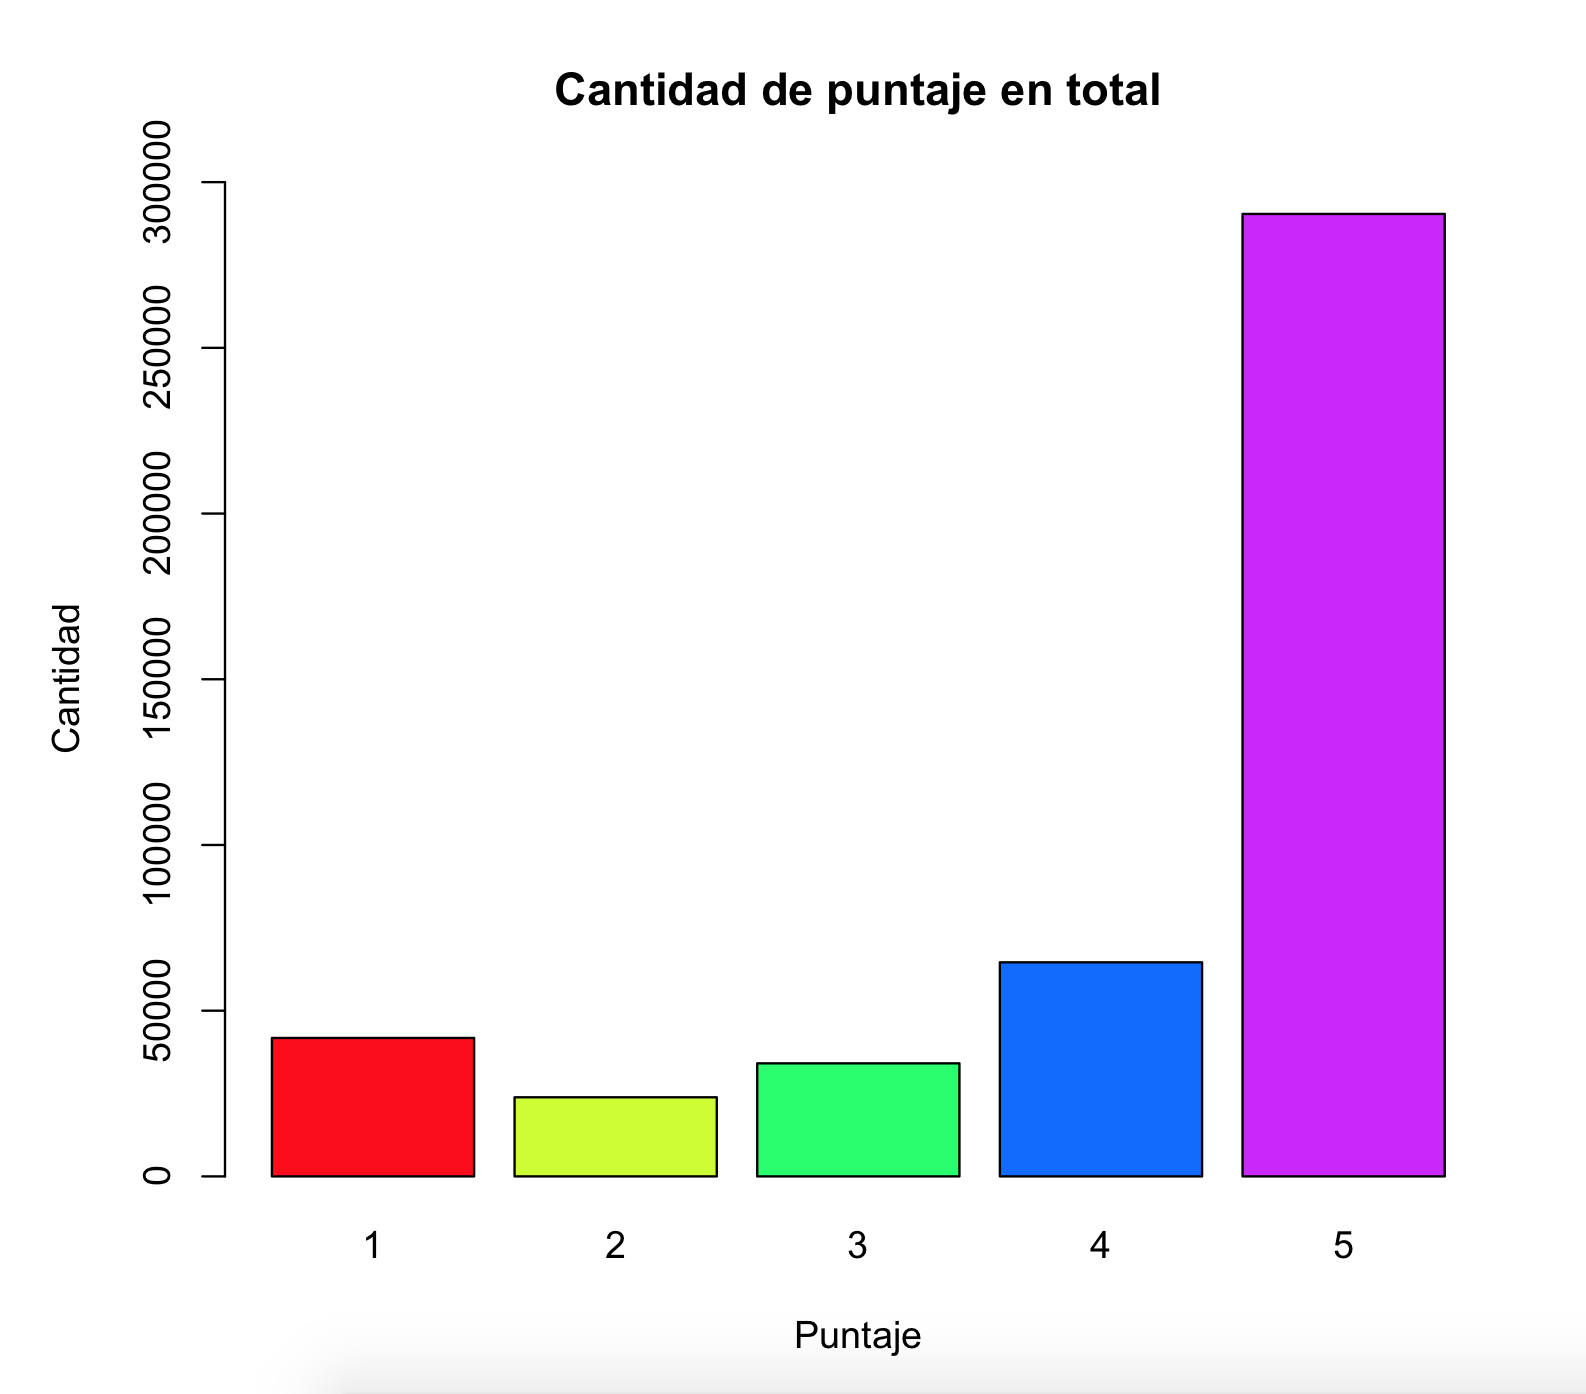
\includegraphics[width=10cm]{puntajcant}
    \caption{Frecuencia de los distintos puntajes}
    \label{fig:2}
  \end{center}
\end{figure}

Se evidencia que hay mayor cantidad de registros con puntajes más elevados, teniendo su valor máximo en los reviews de 5 estrellas. Si bien este dato no es relevante por ahora, nos da una idea de la tendencia de los datos del set. Adicionalmente, en este apartado no se combinaron aún los análisis de cada parámetro por lo que aún no corresponde tomar decisiones e hipótesis apresuradas.

Los últimos campos que quedan por procesar son quizás los más importantes y de mayor peso. Estos son el “Text” y el “Summary” que son del tipo texto por lo que el análisis debe tener otro enfoque. Es aquí donde se ve reflejado el trabajo de Text Mining o más precisaente Opinion Mining y Sentiment Analysis.

\chapter{Transformando los datos}
Nuestro problema puede ser fácilmente formulado como un problema de clasificación, donde se poseen cinco clases (si solo nos limitamos a la puntuación entera) y se debe predecir la clase (puntuación) de una review del set de test en base a un train. Por ende, bien se podría utilizar cualquier algoritmo de aprendizaje supervisado o no supervisado. 

Para que esto sea posible es necesario darle una estructura a un tipo de dato no estructurado como lo es el texto. Es así como la elección del conjunto de features efectivos se vuelve una tarea mas que importante. En nuestro caso nos decidimos por usar términos y sus frecuencias; Cada feature representa a una determinada palabra o a un n-grama y su correspondiente frecuencia. Esperamos a futuro poder utilizar el sistema de ponderación TF-IDF. 
Obviamente tenemos un particular trato los adjetivos y adverbios, ya que son los que definen en gran medida, una review. Por otro lado, las negaciones, también merecen ser tenidas en cuenta, dado que pueden cambiar totalmente la orientación de una review. 
Es entonces que antes de utilizar los datos del set debemos procesar los textos para mejorar el nivel de aprendizaje de los algoritmos y evitar que tome en cuenta palabras o frases perjudiciales para el buen funcionamiento del modelo. Para ello se realizaron las siguientes acciones:
\begin{itemize}
  \item Eliminar signos de puntuación, caracteres especiales y números.
  \item Eliminar “stop words” propias del lenguaje que no aportan nada a la resolución del sentimiento expresado.
  \item Llevar todas las palabras a minúscula para evitar palabras iguales duplicadas por temas de formato.
  \item Detectar las palabras que implican una negación y juntar la frase completa en una sola palabra. Por ejemplo “not good” se llevaría a una sola palabra: “notgood”. Esto es para que una palabra/frase que en principio conlleva un sentimiento negativo como la del ejemplo no sea catalogada como algo positivo por el hecho de tener la palabra “good”.
\end{itemize}

Para las stop words se utilizó una lista de palabras del lenguaje inglés que obtuvimos, la cual fue modificada para que se ajuste mejor a nuestro set de datos. Se le agregaron aquellas palabras poco frecuentes que no aportaban demasiado al análisis de sentimientos.  

\chapter{Combinación de clasificadores}
En general, utilizar mas de un algoritmo es siempre una buena idea a la hora de clasificar algún elemento. Existen diversos métodos para la combinación de clasificadores. Los métodos mas clásicos son el voto por mayoría, el voto por mayoría ponderado, regla de combinación bayesiana, etc. Sin embargo nuestro caso tiene una particularidad y es que es en realidad es un problema de clasificación y a la vez de regresión. Es entonces que decidimos usar un promedio ponderado que tome en cuenta los resultados de los clasificadores y un factor de fiabilidad. 

El factor de fiabilidad es la probabilidad de que un determinado clasificador, determine correctamente la clase de un determinado elemento. Sea $ r_{i} $ el factor de fiabilidad del clasificador i-esimo, pediremos que; $ \Sigma ^{n} _{i = 1} r_{i} = 1 $, donde n es la cantidad de clasificadores. Para obtener este factor utilizaremos una porcion set de train para llevar a cabo pruebas sobre el. Entonces

\[ r_{i} = \frac{C_{i}}{\Sigma ^{n}_{i=1} C_{i}} \]

Donde $ C_{i} $ es la cantidad de elementos que el clasificador i-esimo aserto en su ejecución. $ r_{i} $ es proporcional al nivel de fiabilidad del clasificador i. 

Ahora podemos definir claramente nuestro modelo. Sea $ e_{i}(x) $ la clase a la que el clasificador i adjudico al elemento \textit{x}, decimos que;

\[ Clase(x) = \Sigma _{i=1}^{n}r_{i} . e_{i}(x) \]

En lo que sigue del informe se expondrán distintos métodos de clasificación y su adaptación a nuestro proyecto.

\chapter{Clasificador Probabilistico y Naive Bayes}
La idea consiste en un modelo probabilístico a partir del cual se obtiene un puntaje promedio para cada palabra presente en el set de datos. La fórmula o método utilizado para esto es la siguiente:

\[ Puntaje(Palabra_{i}) = \frac{E_{i}}{T_{i}} \]

Donde $ E_{i} $ es la sumatoria de estrellas de todas las review en donde aparece la palabra i-esima. $T_{i}$ es la cantidad de apariciones de la palabra i-esima.

La clasificación de Bayes consiste en asignarle la clase con mayor probabilidad a un ejemplo determinado a partir de su contenido. Para nuestro caso en particular las clases serían la cantidad de estrellas del review (1,2,3,4 y 5) mientras que los atributos del ejemplo serían cada una de las palabras que compone el texto. De esta forma, la probabilidad de que cada review pertenezca a una de estas clases se generaría de la siguiente forma:
\[ P(C|p_{1}, p_{2},...,p_{n}) = \frac{P(C).P(p_{1}, p_{2},...,p_{n}|C)}{P(p_{1}, p_{2},...,p_{n})} \]

En el modelo de Naive Bayes se asume que cada $ p_{i} $ es independiente de cualquier otra $ p_{j} $ para j distinto de i.  Adicionalmente, En la práctica sólo importa el numerador, ya que el denominador no depende de C y los valores de $ F_{i} $ son datos, por lo que el denominador es constante. Por lo tanto, la ecuación quedaría expreada como: 

\[ P(C|p_{1}, p_{2},...,p_{n}) = P(C).P(p_{1}|C).P(p_{2}|C)...P(p_{n}|C) = P(C).\Pi _{i=1}^{n}P(p_{i}|C)\]

En donde $ P = (p_{1}, p_{2},...,p_{n}) $ son las palabras del texto y C es la clase sobre la cual estamos buscando la probabilidad. 

Luego, la clase a la que va a pertenecer el texto se puede obtener directamente tomando la clase con mayor probabilidad o haciendo un promedio de los valores de las probabilidades de las distintas clases para obtener un número no entero entre uno y cinco.

Los estudios ya realizados y sobre los cuales basamos nuestra decisión son a partir de sentiment analysis que determinan únicamente si el review es positivo o negativo. Nuestro enfoque va más allá de eso e intenta determinar qué puntuación del uno al cinco va a tener cada opinión.

Si bien el modelo que vamos a utilizar se basa en probabilidades y se asemeja al de Naive Bayes, decidimos darle nuestra propia versión al modelo realizando algunos ajuste de procedimiento, incluyendo, por ejemplo, los pesos de los Helpfulness Numbers. Este es uno de los métodos que formaran parte de nuestra solución.

\chapter{K-means y Knn}
Uno de los algoritmos que mas referencias tuvo en toda la bibliografía que revisamos fue sin duda alguna K-means. El algoritmo plantea dividir una colección de n vectores $ {x_{1}, x_{1}, ... , x_{n}} $ en un conjunto de Clusters $ {C_{1}, C_{2}, ... , C_{m}} $. Claramente el primer y tal vez único hiper-parametro (si no tomamos en cuenta el método para medir distancia) que vamos a tener que evaluar. 
Recordamos que estructuramos a cada review como un vector en donde cada componente representa a un termino de su Texto y su frecuencia.
Inicialmente, se necesitan de un conjunto de \textit{m} centroides\footnote{vectores que servirán para formar los Clusters}. Estos pueden ser elegidos tanto de forma aleatoria, entre el conjunto de vectores presentes en nuestro set de Train, como bajo algún criterio especifico, tal como se hace en K-means++\footnote{Se intenta que los centroides iniciales estén lo mas distanciados entre ellos.}
En paso iterativo los centroides $ M_{i} $ de los actuales clusters son calculados de acuerdo a la siguiente formula:
\[ M_{i} = |C_{i}| ^{-1} \Sigma _{x \in C_{i}} x \]
Luego cada vector es reasignado al cluster cuyo centroide sea el mas cercano. Cuando no existan cambios sustanciales en cuanto al centroides entre un paso y otro, la iteracion se detiene.
El algoritmo K-means maximiza la funcion de calidad de cluster \textit{Q}:
\[ Q(C_{1}, C_{2}, ... , C_{m}) = \Sigma _{C_{i}} \Sigma _{x \in C_{i}) Sim(x - M_{i}} \]
Donde la función \textit{Sim} es la inversa de la distancia entre dos vectores. Se entiende entonces que la metrica es un hiper-parametro a tomar en cuenta. 
Podemos utilizar K-means para resolver el problema de Knn de forma eficiente. Recordamos que Knn es un buen algoritmo del cual se hizo referencia en varios textos de la bibliografía estudiada. Pero dada la estructura de datos que utilizamos, no encuentra una solución en un tiempo acotado de ejecución. Sin embargo, si lo combinamos con una variante de K-means llamada K-means Online, puede lograrse una cierto nivel de eficiencia. 


\chapter{Tareas a futuro}
Aun resta testear algoritmos de clasificación que incrementen la precisión de los resultados, pero creemos que dado el modelo que elegimos para nuestros datos, cualquier método sera fácilmente adaptable.

Hacer una investigación acerca de la influencia del contexto en el cual se genera una review. Este tipo de informacion se puede obtener de aquellos campos que descartamos inicialmente como productID, userID, time, etc.

Aun resta realizar algunas mejorar en cuanto al procesamiento de los textos. Puntualmente en separar adjetivos, de adverbios y sustantivos, lo que en Opinión mining llaman extracción de Word Opinion, entidades y aspectos. Y asignar a cada termino un peso distinto en función de su relevancia en una review 

Por ultimo, utilizar n-gramas en el modelo. Esto fue probado en el finger 2 por el grupo para mejorar el resultado de las predicciones con Vowpal Wabbit y las consecuencias fueron muy positivas. Esto se debe a que las palabras por si solas pueden no expresar los sentimientos adecuados para el análisis global de la oración y aún más del review completo.



\begin{thebibliography}{99}
\bibitem{Opinion} Bing Liu, Lei Zhang. A Survey of Opinion Mining and Sentiment Analysis, Capitulo del libro Mining Text Data. Ed. C. Aggarwal, C. Zhai, Springer, 2011.
\bibitem{Comb1} Leah S. Larkey, W. Bruce Croft. Combining Classifiers in text categorization. Departamento de Ciencias de la Computacion. Universidad de Massachusetts.
\bibitem{Poco} Daphne Koller, Mehran Sahami. Hierarchically classifying documents with very few words. Departamento de Ciencias de la Computacion. Universidad de Stanford
\bibitem{mining} Editors: Aggarwal, Charu C., Zhai, ChengXiang (Eds.). Mining Text Data
\bibitem{Com2} Paul N. Bennett, Susan T. Dumais, Eric Horvitz. Probabilistic Combination of Text Classifiers Using Reliability Indicators: Models and Results.
\bibitem{Mining2}Ronen Feldman, James Sanger. The Text Mining Handbook.
\bibitem{Mining3} Kunpeng Zhang, Yu Cheng, Wei-keng Liao, Alok Choudhary. Mining Millions of Reviews: A Technique to Rank Products Based on Importance of Reviews. Universidad de Northwestern.
\bibitem{apunte} Luis Argerich, Apuntes del Curso Organización de Datos.
\bibitem{link1} Data Science in Minutes. 
\url{ https://rdisorder.wordpress.com/2016/08/06/data-science-in-minutes/}
\bibitem{link2} All About Stop Words for Text Mining and Information Retrieval. 
\url{http://text-analytics101.rxnlp.com/2014/10/all-about-stop-words-for-text-mining.html}
\bibitem{link3} Clasificador bayesiano ingenuo. 
\url{https://es.wikipedia.org/wiki/Clasificador_bayesiano_ingenuo}
\end{thebibliography}

\end{document}
